\documentclass[11pt,letterpaper]{article}
\usepackage{babel}
\babelprovide[import,main]{spanish}
\usepackage{fontspec}
\IfFontExistsTF{Arial}{\setmainfont{Arial}\typeout{FUENTE-INFORME: Arial}}{\setmainfont{NimbusSans-Regular.otf}[BoldFont=NimbusSans-Bold.otf,ItalicFont=NimbusSans-Italic.otf,BoldItalicFont=NimbusSans-BoldItalic.otf]\typeout{FUENTE-INFORME: Nimbus Sans}}
\usepackage[margin=2.5cm]{geometry}
\usepackage{booktabs,longtable,tabularx,array}
\usepackage{graphicx,float,setspace,enumitem}
\usepackage[unicode,hidelinks]{hyperref}
\usepackage{xurl}
\usepackage{fancyhdr}
\setstretch{1.14}
\setlength{\parindent}{0pt}
\setlength{\parskip}{7pt}
\setlength{\emergencystretch}{2em}
\setlength{\headheight}{14pt}
\renewcommand{\arraystretch}{1.18}
\AtBeginDocument{\renewcommand{\contentsname}{Contenido}\renewcommand{\tablename}{Tabla}}
\pagestyle{fancy}
\fancyhf{}
\fancyhead[L]{\small MCDI500 · Grupo 7}
\fancyhead[R]{\small Revisión de Formativa 3}
\fancyfoot[C]{\thepage}
\renewcommand{\headrulewidth}{0.2pt}
\renewcommand{\contentsname}{Contenido}
\setcounter{tocdepth}{1}
\newcommand{\Contexto}{revision\_local\_del\_equipo}
\newcommand{\Sistema}{Windows}
\newcommand{\VersionPython}{3.13.15}
\newcommand{\VersionPandas}{3.0.5}
\newcommand{\VersionNumpy}{2.5.3}
\newcommand{\FechaUTC}{2026-09-27}
\newcommand{\NumeroPruebas}{24}
\newcommand{\Ganador}{bucle}
\newcommand{\IntervaloCruce}{entre 1.000 y 2.000 valores}
\newcommand{\HashDatos}{d75de25f676a6c57ddd6f8af19813a6b6ea338e36567c7a096f43e698a49f58e}
\newcommand{\TiempoBucleNativo}{49,56}
\newcommand{\TiempoPandasNativo}{167,43}

\begin{document}
\begin{titlepage}
\thispagestyle{empty}
\begin{center}
\vspace*{1cm}
{\large Universidad Andrés Bello}\par
Magíster en Ciencia de Datos e Inteligencia Artificial\par
MCDI500 — Programación para la Ciencia de Datos\par
\vspace{1.2cm}
{\Large\bfseries Avance de Fase 3}\par
{\large Semana 2 · Revisión de la actividad formativa}\par
\vspace{0.8cm}
{\Large Preparación reproducible de órdenes de Compra Ágil de Valparaíso}\par
\vspace{1cm}
\textbf{Grupo 7}\par
Benjamín Araya Matta\par
Alan Cañete Calquin\par
Patricio Cortez Triviño\par
Jorge Guaico Ortega\par
\vspace{0.6cm}
Docente: Dr. Omar Salinas Silva\par
Entrega original: 25 de septiembre de 2026\par
Revisión técnica: \FechaUTC\par
\vfill
\url{https://github.com/BenjaArayaM/proyecto-grupo7-mcdi500}\par
\vspace{0.4cm}
{\small Correcciones preparadas con asistencia técnica. Los resultados incluidos corresponden a
\Contexto; la revisión y ejecución local del equipo deben registrarse por separado.}
\end{center}
\end{titlepage}
\setcounter{page}{2}
\tableofcontents
\vspace{0.7cm}
\textbf{Alcance de esta revisión.} Se atienden las observaciones recibidas sobre pruebas,
escalamiento, memoria, modularización, arquitectura y redacción. Se conservan la entrada de F2,
las decisiones estadísticas aprobadas y la vinculación con el foro. El documento no presenta
una nueva calificación ni declara concluida la futura sumativa.
\clearpage

\section{Codificación funcional y arquitectura básica}
La revisión conserva las dos estrategias evaluadas: un recorrido con bucle y una selección
vectorizada con pandas. Ambas reciben una serie de montos y dos límites, y devuelven una lista
con los valores estrictamente fuera del intervalo, en su orden original y con sus repeticiones.
El uso de estructuras tabulares se apoya en el enfoque de análisis de datos presentado por
McKinney (2010); la elección de la estrategia se decide aquí mediante mediciones.

La entrega anterior dejaba la carga, la validación y los cuartiles en el notebook. Ahora se
separan en funciones reutilizables: \texttt{cargar\_ordenes} verifica el contrato de entrada;
\texttt{calcular\_limites\_iqr} calcula Q1, Q3, IQR y límites una sola vez; y
\texttt{ejecutar\_benchmark} instrumenta las dos estrategias. El notebook importa esas funciones,
coordina el flujo y explica los resultados. Esta separación permite probar cada responsabilidad
sin depender de variables creadas manualmente en una sesión anterior.

\begin{table}[H]\centering
\caption{Componentes implementados y evidencia verificable}
\begin{tabularx}{\textwidth}{@{}>{\raggedright\arraybackslash}p{6.3cm}X@{}}\toprule
Componente & Responsabilidad \\ \midrule
\path{src/datos_iqr.py} & Localización, lectura y validación de órdenes procesadas. \\
\path{src/funciones_iqr.py} & Validación de serie, límites compartidos y dos filtros. \\
\path{src/benchmark_iqr.py} & Réplicas de carga, tiempo, memoria e intervalos de cambio. \\
\path{tests/test_funciones_iqr.py} & Pruebas ejecutables de contratos, casos límite e integración. \\
\path{notebooks} & Ejecución, tablas, gráficos e interpretación. \\
\path{docs} y \path{evidencias} & Métricas, muestras, informe, pruebas y procedencia. \\
\bottomrule\end{tabularx}
\par\small Rutas relativas a la carpeta F3.
\end{table}

\section{Preprocesamiento y transformación}
La entrada sigue siendo \path{F2/data/processed/ordenes.csv}. F2 transforma el archivo original
de 11.177 filas y 63 columnas en 541 órdenes con atributos de cabecera consistentes. F3 no
repite la limpieza, no trata las filas exportadas como órdenes independientes y no absorbe
las reglas monetarias o de faltantes de F2.

Se seleccionan el código de orden, \texttt{MontoNetoOC\_CLP} y la marca IQR de F2. La conversión
a número utiliza control estricto de errores. Un valor no interpretable, faltante o infinito
detiene el análisis; no se convierte silenciosamente en cero ni se elimina. Los códigos deben
ser no vacíos y únicos. En la base comprobada existen 541 montos válidos y cero faltantes.

Se mantienen todas las monedas y estados porque el monto neto en CLP es la variable comparable
provista por F2. Se conservan las 61 órdenes extremas: una clasificación estadística no
demuestra un error de origen. Se eliminan cero registros y se imputan cero valores. Las
réplicas usadas después para medir carga no se incorporan a este conjunto analítico.

\section{Validación técnica y verificación}
Con interpolación lineal se obtiene Q1 = 217.923 CLP, Q3 = 1.620.152 CLP e IQR = 1.402.229 CLP.
Con factor 1,5, el límite inferior es $-1.885.420,50$ CLP y el superior es 3.723.495,50 CLP.
La interpolación se declara explícitamente para hacer comparable el cálculo con F2
(pandas development team, 2026).

Las dos implementaciones producen la misma lista completa de 61 valores, no solo el mismo
conteo. También coinciden las marcas fila por fila y los códigos de las órdenes identificadas.
La prueba de integración contrasta el nuevo cálculo con \texttt{marcar\_iqr} de F2 y con
los resultados guardados por esa fase. Los límites y los datos de entrada permanecen intactos.

\begin{table}[H]\centering
\caption{Casos cubiertos por las pruebas automatizadas}
\begin{tabularx}{\textwidth}{@{}>{\raggedright\arraybackslash}p{4.3cm}X@{}}\toprule
Caso & Resultado esperado \\ \midrule
Sin valores fuera de rango & Lista vacía en ambos filtros. \\
Todos fuera de rango & Se conservan todos los valores; límites externos $[-1,1]$. \\
Serie vacía con límites conocidos & Lista vacía; no se intentan estimar cuartiles. \\
Estimación con serie vacía & Error explícito: faltan observaciones para Q1 y Q3. \\
Valores iguales a los límites & No son extremos; comparaciones estrictas. \\
Duplicados e índices no consecutivos & Se conserva el orden y la multiplicidad de los valores. \\
Serie constante o de un elemento & IQR cero, sin extremos dentro de su intervalo. \\
Faltantes, infinitos o códigos repetidos & Rechazo antes de medir; no hay corrección silenciosa. \\
Integración con F2 & Mismos límites, 541 OC y 61 extremos. \\
\bottomrule\end{tabularx}
\end{table}

Se ejecutaron \NumeroPruebas{} pruebas de F3 sin fallos, errores ni omisiones en el entorno
declarado. Los casos parametrizados comprueban los dos filtros. La prueba de rendimiento valida
la conservación de muestras y la equivalencia, sin imponer qué implementación debe ganar.
Las evidencias están en \path{F3/evidencias/pruebas_formativa3.json} y su registro de texto.

\begin{figure}[H]\centering
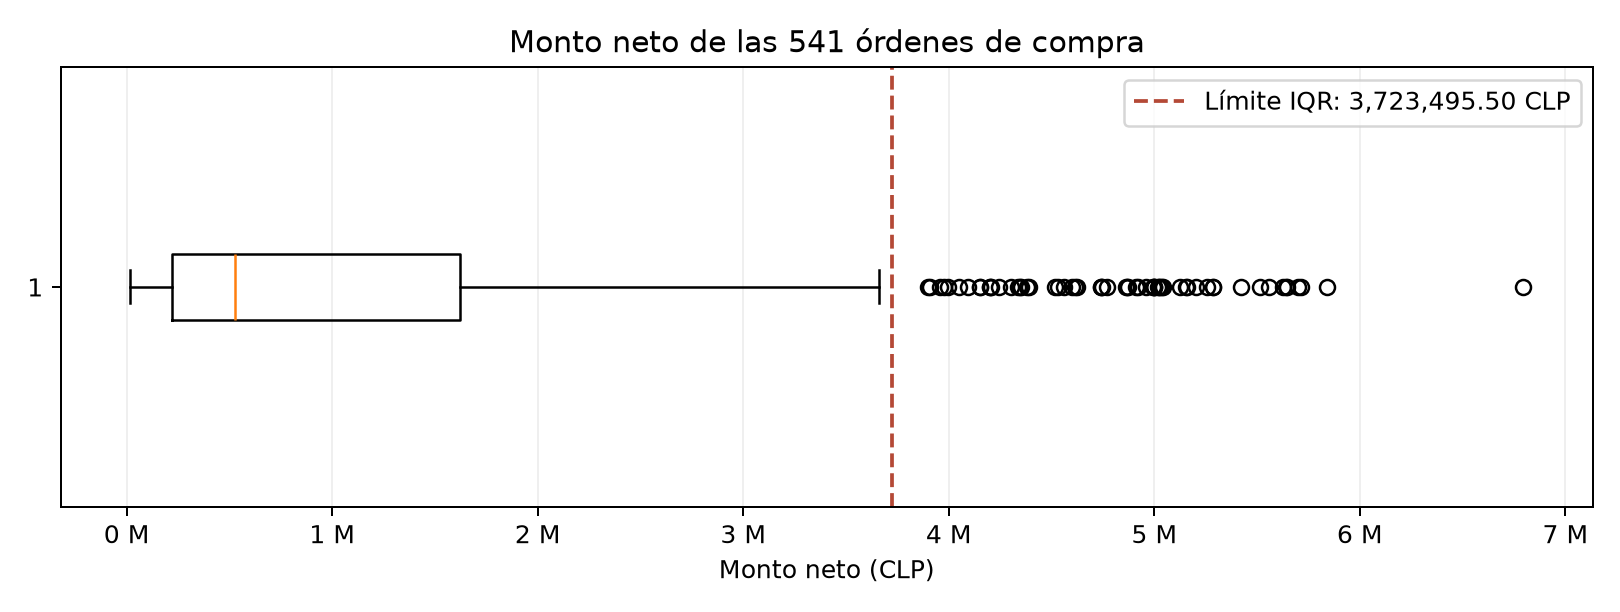
\includegraphics[width=\textwidth]{figuras/distribucion_iqr.png}
\caption{Distribución del monto neto de las 541 órdenes reales.}
\small La línea discontinua señala el límite superior. Los puntos extremos se conservan en F2 y F3.
\end{figure}

\section{Eficiencia y optimización}
\subsection*{Protocolo temporal}
Se preserva el procedimiento aprobado: \texttt{time.perf\_counter}, 1.000 llamadas por medición,
tres mediciones por estrategia y el menor tiempo observado. Se añaden tres llamadas de
calentamiento y alternancia del orden de los métodos para reducir efectos del inicio y del
orden de ejecución. El reloj se elige por su resolución para intervalos breves
(Python Software Foundation, 2026a).

Se evalúan 541, 1.000, 2.000, 5.000, 10.000, 20.000 y 50.000 valores. Los tamaños mayores se
construyen repitiendo cíclicamente la serie y truncándola. Son entradas sintéticas para medir
escalamiento: no constituyen nuevas órdenes ni amplían la evidencia estadística del proyecto.
Los límites obtenidos de las 541 OC permanecen fijos en todos los tamaños.

La lectura, la construcción de réplicas, la validación y los cuartiles se realizan fuera del
intervalo cronometrado. Ambos métodos incluyen la creación de la lista final. Así se compara
la misma tarea y el mismo contrato de salida, manteniendo intactos los cuerpos de los dos
filtros de la entrega. El CSV contiene mínimo, mediana y máximo por llamada; el JSON conserva
las tres mediciones completas de cada combinación.

\subsection*{Protocolo espacial}
La memoria se mide en llamadas separadas, con \texttt{tracemalloc} desactivado durante la
medición temporal. Para cada método y tamaño se registran tres picos incrementales y se
presenta su mediana. La entrada existe antes de iniciar el rastreo y la lista de salida se
mantiene viva al consultar el pico. La medida comprende las asignaciones rastreadas, no la
RAM total del proceso ni necesariamente toda memoria nativa (Python Software Foundation, 2026b).

\begin{table}[H]\centering
\caption{Tiempo por llamada y memoria incremental del experimento actual}
\small\begin{tabular}{rrrrr}
\toprule
Valores & Bucle ($\mu$s) & pandas ($\mu$s) & Bucle (KiB) & pandas (KiB) \\
\midrule
541 & 35,14 & 140,72 & 2,36 & 7,62 \\
1.000 & 66,13 & 142,74 & 4,10 & 10,55 \\
2.000 & 136,06 & 148,49 & 7,63 & 16,97 \\
5.000 & 340,05 & 160,85 & 18,39 & 35,81 \\
10.000 & 682,59 & 174,63 & 36,73 & 67,18 \\
20.000 & 1.378,17 & 210,50 & 71,05 & 129,54 \\
50.000 & 3.431,17 & 302,21 & 178,69 & 317,60 \\
\bottomrule
\end{tabular}

\par\vspace{4pt}\small Tiempo: mínimo de tres mediciones de 1.000 llamadas. Memoria: mediana de tres
picos separados; 1 KiB = 1.024 bytes. Solo la primera fila corresponde al tamaño real de la base.
\end{table}

\textbf{Entorno de estas mediciones:} \Sistema{}, Python \VersionPython{}, pandas \VersionPandas{}
y NumPy \VersionNumpy{}. Contexto: \Contexto.
Estas mediciones corresponden exclusivamente al entorno y al contexto declarados.

\begin{figure}[H]\centering
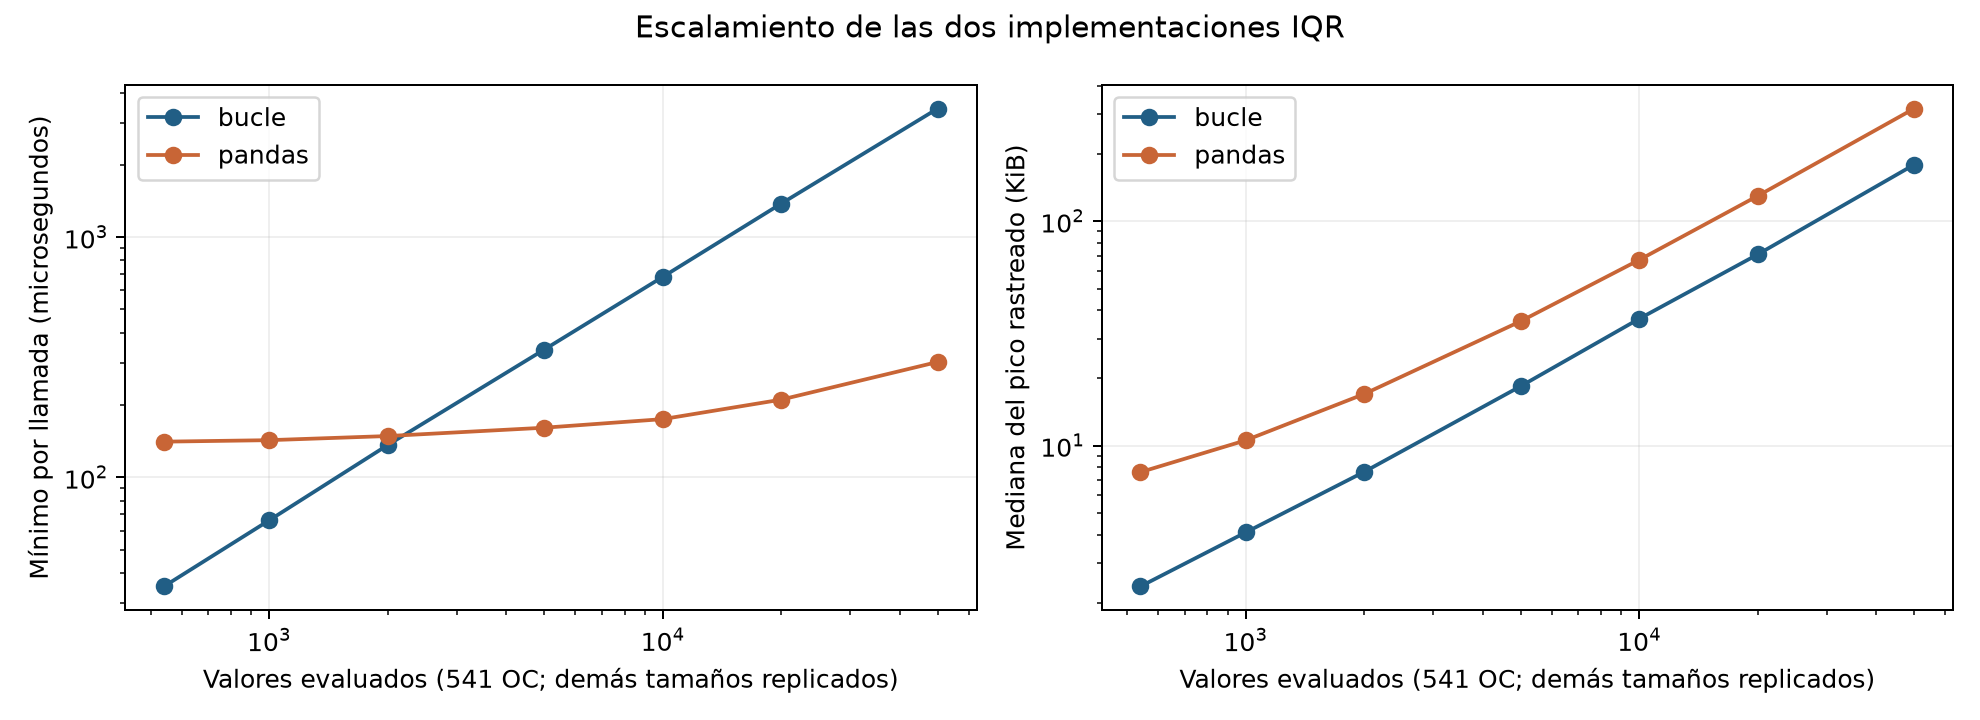
\includegraphics[width=\textwidth]{figuras/tiempo_memoria_iqr.png}
\caption{Escalamiento temporal y espacial en los tamaños medidos.}
\small Ambos ejes usan escala logarítmica para mostrar tamaños pequeños y grandes. Las líneas unen
mediciones y no constituyen un ajuste predictivo.
\end{figure}

\subsection*{Interpretación y decisión}
En la entrega original se observaron aproximadamente 0,033 segundos para el bucle y 0,069
segundos para pandas, por 1.000 ejecuciones sobre 541 valores. Son datos históricos del
notebook entregado y no se presentan como mediciones nuevas. En esta ejecución se obtienen
\TiempoBucleNativo{} y \TiempoPandasNativo{} microsegundos por llamada, respectivamente;
la alternativa más rápida en el tamaño nativo es \Ganador.

Pandas prepara comparaciones, construye máscaras booleanas, combina esas máscaras, selecciona
la serie y convierte el resultado a lista. Ese costo fijo puede pesar más que el ahorro de
recorrido en una entrada pequeña. Con más observaciones, el trabajo vectorizado puede
compensarlo. Esta es una explicación del mecanismo compatible con las mediciones; no se
afirma haber aislado cada operación interna mediante un perfilador.

El cambio de ventaja observado se ubica \IntervaloCruce. El muestreo permite acotar ese cambio,
pero no establece el primer tamaño entero donde ocurre ni garantiza un umbral universal.
En tamaños cercanos deben revisarse la variación entre repeticiones y el entorno de ejecución.
El grupo deberá confirmar su elección con la medición local, conservando las dos estrategias
para que la decisión pueda revisarse sin reescribir la lógica.

Los dos filtros tienen tiempo O(n). El bucle requiere O(k) de memoria para su lista de salida;
pandas añade máscaras y selección O(n), además de la salida O(k), donde k es la cantidad de
extremos. Compartir orden asintótico no implica compartir constantes de tiempo o memoria.
Estas cotas se refieren al filtrado, no al algoritmo interno de cuantiles ni a todo el pipeline.

\section{Diseño estructurado del código}
Se mantiene el argumento aprobado sobre recursión. El problema consiste en recorrer una
serie plana y comparar cada elemento con dos límites conocidos; tiene una secuencia de
pasos definida y no requiere explorar estructuras anidadas de profundidad desconocida.
La división funcional permite explicar, probar y cambiar cada paso sin añadir llamadas recursivas.

La decisión depende de la naturaleza del problema. Si posteriormente se incorporan jerarquías
o procesos de profundidad variable, se reevaluará la recursión. No se agrega por cumplir una
preferencia de estilo: la rúbrica admite división funcional y/o recursividad.

\section{Implementación modular y organización del código}
F2 conserva sus 17 funciones de preparación. F3 tenía inicialmente dos funciones de detección;
esta revisión extiende esa base con validación, límites compartidos y un módulo de medición.
La evolución responde a problemas concretos de la entrega: cuartiles repetibles fuera del
notebook, entrada verificable y pruebas que se ejecutan directamente desde Python.

No se trasladan las reglas de F2 a un módulo nuevo. El archivo procesado y las métricas son
la interfaz entre fases. La prueba contra \texttt{marcar\_iqr} comprueba continuidad; la segunda
implementación del criterio existe para comparar estrategias y no para redefinir la limpieza.
Si en el futuro se extrae una utilidad compartida entre fases, esa refactorización requerirá
pruebas de regresión de ambas para evitar cambios retrospectivos inadvertidos.

Las funciones no necesitan mantener estado entre ejecuciones, por lo que se conserva el
enfoque funcional admitido en esta formativa. La organización facilita una evolución posterior
a POO cuando la guía correspondiente exija o justifique objetos, sin crear aquí una jerarquía
artificial. Esta distinción respeta el alcance del avance y el material del curso
(Universidad Andrés Bello, 2026a, 2026b).

\section{Documentación de arquitectura}
La arquitectura separa preparación de datos, cálculo estadístico, instrumentación y comunicación
de resultados. Esta decisión evita que cambiar el protocolo de tiempos cambie el criterio de
atipicidad, y que modificar una visualización obligue a tocar la limpieza de F2.

Se descarta concentrar todo en el notebook porque impediría probar de forma aislada la lectura
y los contratos. También se descarta copiar F2 dentro de F3: crearía dos versiones de las
reglas monetarias y de faltantes. Conservar módulos por responsabilidad y un contrato explícito
reduce ese riesgo y permite revisar la continuidad mediante pruebas.

La salida de los filtros permanece como lista porque esa era la interfaz evaluada. Conserva
valores, orden y multiplicidad, pero no el índice. Para sostener trazabilidad por orden se añade
un contraste específico de máscaras y códigos, en vez de atribuir a la lista información que
no contiene. El detalle de alternativas y consecuencias está en \path{F3/docs/arquitectura.md}.

La evolución propuesta es gradual: primero validar contratos y resultados; después elegir una
estrategia según las mediciones; finalmente incorporar objetos o una utilidad común si los
requisitos posteriores lo demandan. Los datos sintéticos de rendimiento nunca se reutilizarán
como nuevas observaciones de entrenamiento.

\section{Notebooks ejecutables}
El notebook corregido contiene nueve celdas de código, con narrativa para cada etapa y salidas
conservadas. El ejecutor inicia un proceso nuevo, verifica contadores consecutivos, detiene la
ejecución ante errores y registra los hash del notebook, de los módulos y de las pruebas.
La etiqueta de contexto y las versiones proceden de la ejecución real.

Se conserva la referencia al foro técnico incluida en la entrega: las decisiones de diseño se
fundamentan en la naturaleza del problema y en evidencia de eficiencia, no en asumir que una
estrategia gana siempre. La revisión amplía esa discusión con tamaños crecientes, memoria y
contratos verificables. No se inventan nuevas intervenciones de integrantes en el foro.

La ejecución se reproduce con \texttt{python scripts/ejecutar\_formativa3.py}. El verificador
comprueba que los datos y el código corresponden a las evidencias antes de compilar el PDF.
Los tiempos pueden variar entre máquinas aunque las 541 OC, los límites y los 61 extremos
deban permanecer consistentes. El informe se genera desde las métricas, evitando transcribir
manualmente los resultados del benchmark.

\section{Repositorio GitHub}
La revisión se preparó en una copia independiente del estado \texttt{c02beb5} de \texttt{main}.
No se crearon ramas, commits ni pull requests durante la preparación. El grupo debe revisar,
aplicar, ejecutar y publicar los cambios desde su equipo. El historial de publicación solo
existirá cuando esos pasos se hayan realizado efectivamente.

Se incorporan pruebas reales en la carpeta antes vacía, documentación de decisiones y un README
que identifica el procedimiento de reproducción. Se prepara un archivo \texttt{.mailmap} para
los dos pares de alias comprobados con el mismo correo. Esto normaliza la presentación de
autores en herramientas compatibles sin reescribir commits ni cambiar sus fechas.

Para atender la observación sobre documentos duplicados, el tutorial indica retirar el Word
del índice de Git mediante \texttt{git rm --cached}, conservándolo localmente. El PDF es el
documento de entrega. La fuente LaTeX se conserva como código de generación reproducible;
no es una segunda versión editorial independiente del informe.

Además, se reparan por separado dos archivos de F2 que contenían marcas de conflicto:
el notebook y el JSON de entorno. Se recupera la variante histórica \texttt{Updated upstream},
sin cambiar el código de preparación ni atribuir esa evidencia histórica a una ejecución nueva.
La copia original se respalda antes de aplicar el paquete. Las 18 pruebas de F2 pasaron en la
comprobación asistida; ello no sustituye la revisión local del equipo.

\clearpage
\section{Referencias}
\begin{list}{}{\setlength{\leftmargin}{0.65cm}\setlength{\itemindent}{-0.65cm}\setlength{\itemsep}{9pt}}
\raggedright
\item McKinney, W. (2010). Data structures for statistical computing in Python. En
\textit{Proceedings of the 9th Python in Science Conference} (pp. 56–61).
\url{https://doi.org/10.25080/Majora-92bf1922-00a}
\item pandas development team. (2026). \textit{pandas.Series.quantile}. pandas documentation.
\url{https://pandas.pydata.org/docs/reference/api/pandas.Series.quantile.html}
\item Python Software Foundation. (2026a). \textit{time — Time access and conversions}.
Python documentation. \url{https://docs.python.org/3/library/time.html}
\item Python Software Foundation. (2026b). \textit{tracemalloc — Trace memory allocations}.
Python documentation. \url{https://docs.python.org/3/library/tracemalloc.html}
\item Universidad Andrés Bello. (2026a). \textit{MCDI500: Apunte Fase 3} [Material del curso].
Magíster en Ciencia de Datos e Inteligencia Artificial.
\item Universidad Andrés Bello. (2026b). \textit{MCDI500 Fase 3, Semana 2: Núcleo algorítmico,
eficiencia y programación orientada a objetos} [Material del curso]. Magíster en Ciencia de
Datos e Inteligencia Artificial.
\end{list}
\vfill
{\small Nota de reproducción: este PDF corresponde al contexto \Contexto. En Windows, XeLaTeX
usa Arial si está disponible. La revisión de Linux usa Nimbus Sans como sustitución; la
fuente utilizada queda registrada en la evidencia de compilación.}
\end{document}
